\documentclass[11pt]{article}  
\usepackage[T1]{fontenc}
\usepackage[utf8]{inputenc}
\usepackage{helvet}
\usepackage{titlesec} 
\usepackage[frenchb]{babel}
\usepackage{amsmath,amssymb}
\usepackage{tabu}
\usepackage[svgnames]{xcolor}
\usepackage{graphicx}
\usepackage{geometry}
\usepackage{layout}
\usepackage{listings}
\usepackage{textcomp}
\usepackage{minted}
\usepackage{pdfpages}
\usepackage{fancyhdr}
\usepackage{lastpage}

\newenvironment{strechpage}[1][0cm]{%
	\newpage\vspace*{#1}\leavevmode\noindent\centering
	\def\tempdimen{#1}%
	\begin{minipage}{\dimexpr\linewidth-#1-#1\relax}}%
	{\end{minipage}\vspace*\tempdimen\newpage}
	
\pagestyle{fancy}
\renewcommand\headrulewidth{1pt}
\fancyhead[L]{TER: Calcul GRID avec de la messagerie instantanée}
\fancyhead[R]{URCA}
\renewcommand\footrulewidth{1pt}
\fancyfoot[L]{HERARD Joffrey}
\fancyfoot[C]{
\textbf{Page \thepage/\pageref{LastPage}}}
\fancyfoot[R]{2016-2017}



\titleformat{\chapter}[display]
  {\centering\normalfont\huge\bfseries}
  {\chaptertitlename\ \thechapter}
  {20pt}
  {\Huge}
  
\newcommand\T{\rule{0pt}{2.6ex}}       % Top strut
\newcommand\B{\rule[-1.2ex]{0pt}{0pt}} % Bottom strut

\begin{document}
 \makeatletter
\def\maketitle{%
  \null
  \thispagestyle{empty}%
  \vfill
  \begin{center}\leavevmode
    \normalfont
    {\Huge \@title\par}%
    \vskip 3cm
    {\Large \@author\par}%
    \vskip 1cm
    {\Large \@date\par}%
  \end{center}%
  \vfill
  \null
  \cleardoublepage
  }
\makeatother
\title{Solution générique de calcul GRID exploitant des messageries instantanées
(Java / Python, XML, XMPP / IRC)}
\author{ Réalise par Joffrey Hérard \begin{center}Responsable : Olivier Flauzac\end{center}}
\date{2016-2017}
\maketitle
 
\tableofcontents 

\newpage
\section{Introduction} 
Sujet : Solution générique de calcul GRID exploitant des messageries instantanées
(Java / Python, XML, XMPP / IRC)
Durant ce TER, il a été demandée la mise en place d'un système de calcul repartie entre plusieurs machines avec l'évaluation de possibilité d'exécutions ou non par la machine cible, il fallait aussi évaluer quels échanges allais être réalise par les acteurs durant une exécution type et ceci en avec le protocoles XMPP ou IRC. Il seras détaillé dans ce rapport l'ensemble des échanges ainsi que l'ensemble des gestions d'erreurs déployé. 
\newpage
\section{Les Acteurs} 
Nous avons donc deux genres d'acteur pour chaque travail différent disponibles 
\begin{itemize}
\item Fournisseur de travail/Provider, unique pour chaque travail.
\item Des travailleurs/Workers, de 1 a n, n définit par le problèmes.
Chaque Provider est possiblement exécuter sur n'importe quel système d'exploitation  tout comme chaque worker
\item Un serveur XMPP qui sert de support a la messagerie instantanée avec Openfire.
\end{itemize}
\newpage

\section{Les Échanges} 
Voici la liste des différents message qui transitent a travers une exécution type.

 
\begin{enumerate} \item Nous avons en premier le message de type "ENVOI JOB" il contient :
\begin{itemize}
\item l'identifiant du problème,
\item Le code des contraintes,
\item Le code a exécuter,
\item La ligne de  commande pour l\textquoteright exécuter.
\item Le nom du fichier à exécuter.
\end{itemize}

\item Ensuite il y a le message ou le workers signale qu'il est prêt il contiens juste un message pour signale dans une chaîne de caractère " Je suis prêt".
\item Il y a enfin le message qui renvoi le résultat "REPONSE JOB" il contient : 
\begin{itemize}
\item L'identifiant pour savoir si le code a pu être exécute.
\item L'identifiant du problème.
\item La valeur du retour de l\textquoteright exécution.
\item Code de contraintes, si on a pas pu exécuter .
\item Code exécutable, si on a pas pu exécuter .
\item Ligne de commande associe,  si on a pas pu exécuter .
\item Le nom du fichier à exécuter.
\end{itemize}
\end{enumerate}
Voici la liste des fichiers schéma XML associe ainsi que leurs locations au sein du projet :
\begin{itemize}	
\item "ENVOI\_JOB" = ../Schema\_XML/ENVOI\_RECEPTION.xsd.
\item "REPONSE\_JOB"= ../Schema\_XML/JOB\_REP.xsd.

Tout les codes du projet sont présenter en annexe.
\end{itemize}



\newpage

 
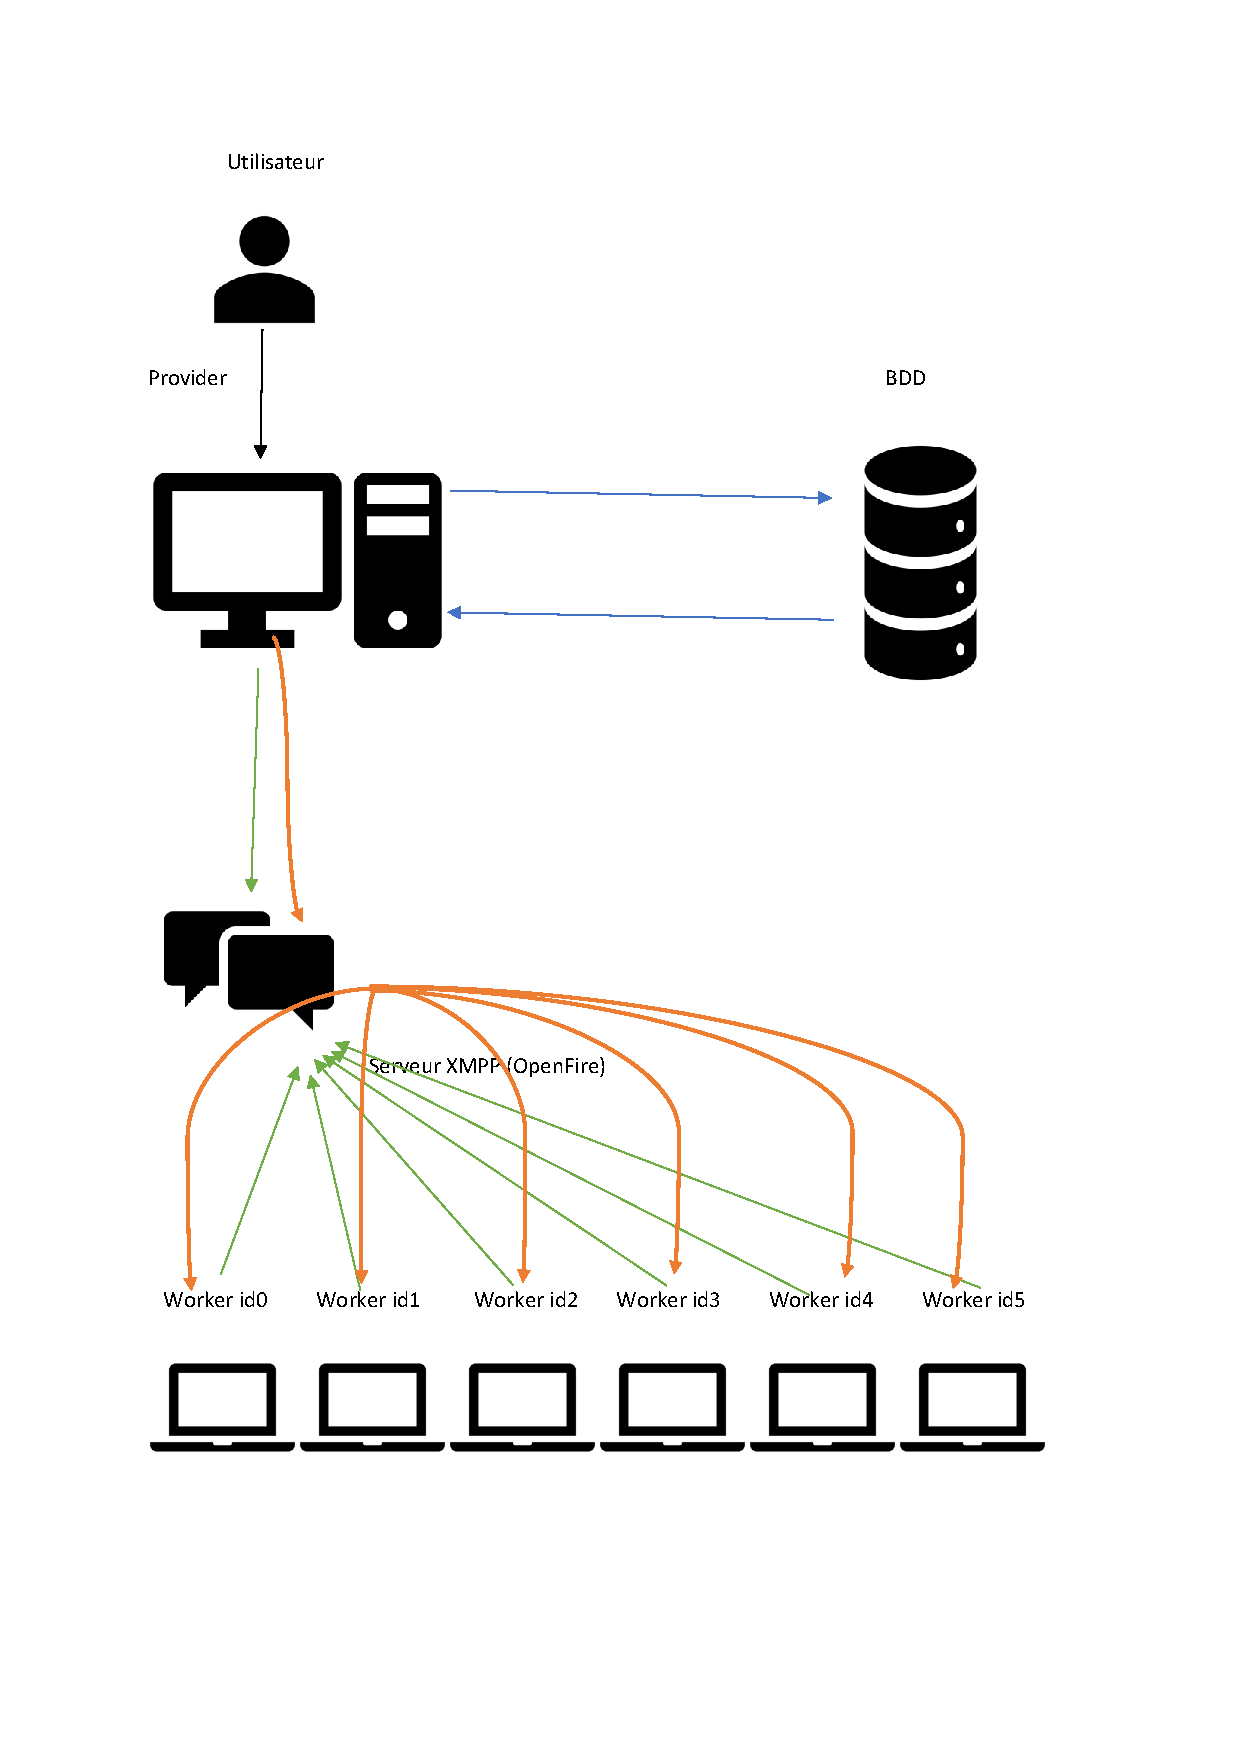
\includepdf[scale=0.7,pages=1,pagecommand=\section{Modélisation}\subsection{Schéma général}\subsubsection{Schéma global d'envoi d'un job}]{toto.pdf}
\includepdf[scale=1,pages=4]{toto.pdf}

\includepdf[scale=0.7,pages=2,pagecommand=\subsubsection{Schéma global d'envoi de réception d'un job}]{toto.pdf}
\includepdf[scale=1,pages=3]{toto.pdf}
\newpage
\subsection{Représentation des JOBS}
Nous allons dans cette partie du rapport montrer la représentation nécessaire et désirer pour représenter un travail.Donc un problèmes c'est quoi? 

\begin{itemize}
\item Identifiant d'un problème, un entier de 0 a n.
\item Code de contraintes, ce code est forcement un code Perl avec un code de retour bien particulier 0 pour non exécutable  et 3 pour exécutable et donc que l'on peut exécuter. 
\item Type du fichier par exemple ".c , .cpp, .cc, .java , .pl etc.."
\item Code d'exécution, peut importe son langage. on peut l'exécuter si le code contraintes l'a valider 
\item La ligne de commande pour exécuter le code par exemple "perl monfichier.pl"
\end{itemize}

\inputminted{XML}{../Schema_XML/BDD_JOB.xsd}
\newpage 

\subsection{Représentation des fichiers de lignes de commandes} 
Chaque ligne de commande doit être représenter comme elle se doit de respecter ces 2 regles simple 
c'est a dire 
\begin{enumerate}
\item Après la commande de type perl, python. ./, il doit être suivit d'un @,  
\item La commande puis une ','
\end{enumerate}
Si ces règles ne sont pas respect, le "parsing" se faisant sur ce fichier par une expression régulière ne s\textquoteright appliquera pas correctement  
\inputminted{perl}{../Echantillon_Script_Cmd/Toto.dc}
Exemple de Langford\_mono12.dc :
\inputminted{perl}{../Echantillon_Script_Cmd/Langford_mono12.dc}
Exemple de nQueen14.dc :
\inputminted{perl}{../Echantillon_Script_Cmd/nQuenn14.dc}

La raison principale de la présence de l'arobase c'est que il va falloir reconstruire la ligne de commande pour ajouter le chemin correspondant.
La raison de la présence de la virgule c'est la ligne de commande personnalise d'un worker séparer d'une autre .
\newpage
\subsection{Les différentes fonctions principales}

\subsubsection{Contraintes} 
L'execution d'un script de contrainte ce fait avec les objets Runtime et Process on obtient le résultat du script avec la fonctin waitFor() 
\inputminted{perl}{../Echantillon_Script_Perl/OSname.pl}
\newpage
\subsubsection{Séparation} 
La fonction split peut se résumer en plusieurs étapes, premièrement on récupère tout les nickname et JID de chaque utilisateur de la chatroom ,pour chacun d'entre eux on leur envoi un fichier xml personnalise avec chacun une tache bien distincte en respectant le schéma associe.Pour avoir une trace on sauvegarde chaque fichier xml envoyer dans le dossier JOB\_SEND
\inputminted[tabsize=2,frame=lines,linenos]{java}{Fichier_import/split.java}
\subsubsection{Exécution} 
L\textquoteright exécution d'un script d'exécution ce fait avec les objets Runtime et Process on obtient le résultat du script avec la fonctin waitFor() bien entendu on parle de calcul chiffrer ,cela peut être aussi un résultat chiffre dans un fichier. 
\inputminted[tabsize=2,frame=lines,linenos]{Perl}{Fichier_import/calcul.pl}
\newpage
\subsubsection{Construction du résultat} 
La fonction build est simplement une addition de chaque résultat reçu petit a petit 
\inputminted[tabsize=2,frame=lines,linenos]{java}{Fichier_import/build.java}
\newpage
\subsection{Description d'une exécution quelconque} 
\subsubsection{Exécution cote Provider}
Voici un déroulement classique cote Provider :
\begin{enumerate}
\item Un Provider choisi un problème a lancer.
\item Une fois le Problème lancer une Chatroom comportant le nom du problème+Providingroom est créer sur le domaine
\item Le Provider attend un nombre suffisant de Worker en fonction du probleme(champ rang du XML)
\item Une fois un nombre de Worker atteints, on récupère chaque identifiant et on leur envoi leur job respectif et ligne de commande respective
\item On attend d'avoir reçu un message de type "JOB\_Reponse" autant de fois et distinct que de Workers capable de l'exécuter 
\item On affiche le résultat
\end{enumerate}

\subsubsection{Exécution cote Worker}
Voici un déroulement classique cote Worker
\begin{enumerate}
\item On s'identifie
\item On choisi un salle de travail 
\item une fois connecter on applique la même routine 
\item A savoir, on exécute chaque script de contrainte si ils sont valide on exécute le fichier exécutable avec la ligne de commande associe.
\end{enumerate}
\subsubsection{Exécution d'un ajout}
\begin{enumerate}
\item On demande le nom du problème 
\item On demande en entrer le chemin absolu pour un fichier de contrainte
\item On demande en entrer le chemin absolu pour un fichier exécutable
\item On demande en entrer le chemin absolu pour un fichier correspondant aux ligne de commande
\item On demande en entrer un rang qui est égale aux nombre de workers nécessaire 
\item Tout ceci est ajouter a un fichier XML nomme nom\_du\_probleme.xml
\end{enumerate}

\newpage\subsubsection{Exécution d'une suppression}
\begin{enumerate}
\item On demande le nom du problème 
\item On supprime le fichier XMl associe 
\end{enumerate}
\newpage
\section{Formatage des fichiers sources décrivant un JOB}
\subsection{Script de contraintes}
\subsubsection{Principe}
Tout script de contraintes doit répondre a ces propres contraintes :
\begin{enumerate}
\item Être écrit en Perl
\item Avoir un retour de commande avec "exit(3);" pour un retour validant la poursuite du processus 

\end{enumerate}
\subsubsection{Exemple}
\subparagraph{Exemple pour un programme interpréter}
Pour un langage interpréter comme le python en voici un exemple
\inputminted{perl}{../Echantillon_Script_Perl/nqueen.pl}
\subparagraph{Exemple pour un programme compilé }
Quand il s'avère que vous devez valide la compilation puis sa future exécution d'un code exécutable tel q'un code de langage compilé comme le C en voici un exemple sur comment faire 
\inputminted{perl}{../Echantillon_Script_Perl/langford.pl}
\subsection{Script de Commandes}
\subsubsection{Principe}
Cette partie fait aussi une référence, voir une redite avec le section 5-3. Tout script de commande doit répondre a ces propres contraintes:
\begin{enumerate}
\item Après la commande faisant appelle a un interpréteur mettre le caractère "@"
\item Dans le cas d'un split a plus de 1 Worker, utiliser les virguler pour séparer chaque commande approprie pour chaque worker
\item Les caractères évidemment interdit sont : @, ',', [, ] .en raison d'exploitation d'expression régulière.
\end{enumerate}
\subsubsection{Exemples}
Voici quelques exemples :
\inputminted{perl}{../Echantillon_Script_Cmd/nQuenn14.dc}
\inputminted{perl}{../Echantillon_Script_Cmd/Toto.dc}

\subsection{Script d'execution}
\subsubsection{Principe}
Tout script des exécutions doit répondre a ces propres contraintes :
\begin{enumerate}
\item Avoir connaissance que toutes les données renvoyer par les Worker seront passée dans le fichier resultat.
\item Écrire le résultat dans un fichier "resultat.txt".
\end{enumerate}


\subsection{Script de build}
\subsubsection{Principe}
Tout script de construction doit répondre a ces propres contraintes :
\begin{enumerate}
\item Être écrit en Perl.
\item Avoir connaissance que toutes les données renvoyer par les Workers seront passée en argument.
\item Écrire le résultat dans un fichier "resultatF.txt".
\end{enumerate}
\subsubsection{Exemple}
\inputminted{perl}{../Echantillon_Script_build/build.pl}
\newpage
\section{Contrainte du serveur OpenFire }
Il est nécessaire afin que le programme fonctionne que le serveur soit accessible par toute personne de la ou elle se trouve, il est possible de demander une machine virtuelle avec un serveur OpenFire(ou autre d’ailleurs) tant que il est possible pour un provider d'y être inscrit par un administrateur au grade de modérateur, respectivement pareil pour un worker. 
I lest important de savoir que la il y a plusieurs limite de OpenFire.
\newpage
\section{Les Erreurs} 
\subsection{Les Problèmes d'exécution}
Les problèmes qui peuvent opérer a travers le système,sont : 
\begin{enumerate}
\item Mauvais nom de domaine 
\item Problème de Chatroom déjà existante
\item Problème d'exécution : aucun worker peut exécuter le code, comment le détecter?

\end{enumerate}  

\newpage
\subsection{Les Problèmes réseaux}
Nous avons plusieurs problèmes lie au réseaux quelque soit le protocole utilise :
\begin{enumerate}
\item Latence/Impossible a établir une  connexion a la Chatroom
\item Latence/Impossible a envoyer un  message d'un Provider vers un Worker
\item Latence/Impossible a envoyer un  message d'un Worker vers un Provider
\item Un Worker est déconnecte en plein milieu de sa tache
\item Un Provider est déconnecte durant l'attente d'une réponse sur un JOB
\end{enumerate}


\newpage
\subsection{Gestions des erreurs}

\subsubsection{Gestions des erreurs sur l\textquoteright exécution}
\begin{enumerate}
\item Mauvais nom de domaine $ \rightarrow $ Redemander le nom de domaine jusqu'à validation .
\item Problème de Chatroom déjà existante $\rightarrow$ Message d'erreur un problème exactement identique est en cours d'exécution .
\item Problème d'exécution : aucun worker peut exécuter le code, comment le détecter? $\rightarrow$ Mis en place d'un tableau de variable booléenne au départ initialise a faux, si un worker renvoi avec une impossibilité d\textquoteright exécution du code dicte par le code contrainte, alors on met a vrai et on redistribue. Si aucun est capable on arrête l\textquoteright exécution.
\end{enumerate}  
\subsubsection{Gestions des erreurs sur le réseaux}
\begin{enumerate}
\item Latence/Impossible a établir une  connexion a la Chatroom$ \rightarrow $ Message qui explicite le fait d'aller voir un Administrateur Reseaux
\item Latence/Impossible a envoyer un  message d'un Provider vers un Worker$ \rightarrow $ Message qui explicite le fait d'aller voir un Administrateur Réseaux
\item Latence/Impossible a envoyer un  message d'un Worker vers un Provider$ \rightarrow $ Message qui explicite le fait d'aller voir un Administrateur Réseaux 
\item Un Worker est déconnecte en plein milieu de sa tache$ \rightarrow $ Détecteur de présence permis par le protocole XMPP sur une ChatRoom MultiUser
\item Un Provider est déconnecte durant l'attente d'une réponse sur un JOB$ \rightarrow $ Évaluation de présence d'un Provider, si aucun alors arrêter le Job en cours, ou mis en place d'un Timeout.
\end{enumerate}

\newpage
\section{Conclusion}
Cette conclusion seras séparer en plusieurs partie la premier concernant l'aspect des problèmes qui resterais a gérer. La deuxième partie seras concentre sur la partie XMPP la troisieme sur IRC, et la quatrième sur une virtualisations des services. Pour finir cette conclusion, un retour sur le TER.
\subparagraph{Les problèmes qui reste a gérer}
\begin{enumerate}
	\item Comment résoudre une perte réseaux  de longue durée sur un worker, quels-serait la pertinence d'un envoi de résultat après un certain temps? 
	\item Avoir des informations de disponibilité de la bande passante du serveur hôte de messagerie instantanée si l'on souhaite avoir des communications en temps réels.
	\item Si le Provider de JOB tombe en panne pendant les calculs que faire, que ce soit un problème réseaux ou électrique. 
\end{enumerate}
\subparagraph{OpenFire}
\begin{enumerate}
\item Il reste a évaluer les besoins et la montée en charge associe au serveur XMPP. Il aurait été plus intéressant lors de mes tests, d'utiliser un serveur XMPP externe pour lui faire éprouve des stress test.Ainsi donc en voir des éventuelle limites qui apporterait de nouveau problèmes a gérer 
\item Il y a des machines virtuelles avec des serveur XMPP déjà configure c'est une vois qu'il reste a exploite 
\end{enumerate}

\subparagraph{JOB a entrevoir} 
Comme nous en avons déjà parler durant quelque entrevue, il reste un point sur lequel je n'ai pu me pencher une utilisation par exemple de l'outil POV-ray ou des tabulations de Golomb. Respectivement, POV-ray s'utilisant en lignes de commandes , seul le support de travail reste a définir, Les tabulations de Golomb sont particulières, elle reste du domaine du calculatoire sur les espacements de blocs. 
\subparagraph{Virtualisation des services}
Une possibilité qui techniquement était envisageable sur ce sujet de TER,  il est possible de lancer des conteneurs par exemple avec Docker.Évidemment L’intérêt serait d'avoir des machines personnalises avec les outils qui serait intéressant. Tout cela j'ai pu les envisager avec l'aide de Guillaume Bourgeois, qui m'as conseille sur la manière de les gérer, je n'ai évidemment pas développer en profondeur cela dans le désir de ne pas empiéter sur son sujet.
\subparagraph{En résumé } 
Le sujet avait beaucoup d'aspect a couvrir, bien entendu tout l'aspect réseau, pour la transmission des messages, l'aspect programmation pour s'adapter aux API XMPP disponible, et bien entendu l'aspect d’études sur les échanges, et la montée en charges  des besoins pour le serveur XMPP.

\newpage

\section{Annexes}
\subsection{Organisation du dossier du projet}
\begin{itemize}
\item / \begin{itemize}
		\item /bin  \begin{itemize} \item Tout les fichiers .class \item Images \item Schema    \end{itemize}
		\item /DB\_JOBS \begin{itemize} \item Calculatoire.xml \item LangfordMono12.xml \item NQueenMono8build.xml \ \item Tout les probleme.xml \end{itemize}
		\item /Echantillon\_Script\_Cmd \begin{itemize} \item Toto.dc \item nQueen14.dc \item Langford\_mono12.dc\item Tout les probleme.dc\end{itemize}
		\item /Echantillon\_Script\_Exec \begin{itemize}\item calcul.pl \item Langford(Dossier comportant les fichiers exemple sur langford) \item nQueen(Dossier comportant les fichiers exemple sur nqueen)  \end{itemize}
		\item /Echantillon\_Script\_Perl \begin{itemize}\item  OSname.pl \item nqueen.pl \item langford.pl\end{itemize}
		\item /JDOM  
		\item /JOB\_REC \begin{itemize}\item /DATA\_EXTRACT \begin{itemize} \item fichier\_extraits\end{itemize}\item xml\_receive.xml  \end{itemize}
		\item /JOB\_SEND \begin{itemize}\item XML\_send\_0.xml \end{itemize}
		\item /openfire
		\item /Rapport \begin{itemize}\item TER\_Joffrey\_Herard.pdf  \end{itemize} 
		\item /Schema\_XML \begin{itemize}\item BDD\_JOB.xsd \item ENVOI\_RECEPTION.xsd \item JOB\_REP.xsd \end{itemize}
		\item /smack\_3\_1\_0
		\item /src \begin{itemize}\item Tout les fichiers .java \end{itemize}
		\item README.md 
\end{itemize}

\end{itemize}
\newpage
\subsubsection{Outils et langages} 
\begin{enumerate}
\item Le projet a été programme en Java version : "1.8.0\_111" sous Eclipse  .
\item L'API smack a été utilisé pour mettre ne place les échanges sous XMPP.
\item Openfire a été utilisé pour installer un serveur XMPP en local afin d'exécuter tout les test.
\end{enumerate}
\newpage

\newpage
\subsection{Code}
\subsubsection{XML} 

BDD\_JOB.xsd
\inputminted[tabsize=2,frame=lines,linenos]{XML}{../Schema_XML/BDD_JOB.xsd}

ENVOI\_RECEPTION.xsd
\inputminted[tabsize=2,frame=lines,linenos]{XML}{../Schema_XML/ENVOI_RECEPTION.xsd}
\newpage
JOB\_REP.xsd
\inputminted[tabsize=2,frame=lines,linenos]{XML}{../Schema_XML/JOB_REP.xsd}
\newpage
\subsubsection{Fichier de lignes de commande .dc}
Les exemple de fichier de commande écrit en texte clair 
Toto.dc
\inputminted[tabsize=2,frame=lines,linenos]{Perl}{../Echantillon_Script_Cmd/Toto.dc}
\subsubsection{Perl}
Les exemple de fichier de contrainte écrit en Perl 
langford.pl
\inputminted[tabsize=2,frame=lines,linenos]{Perl}{../Echantillon_Script_Perl/langford.pl}

nqueen.pl
\inputminted[tabsize=2,frame=lines,linenos]{Perl}{../Echantillon_Script_Perl/nqueen.pl}
OSname.pl
\inputminted[tabsize=2,frame=lines,linenos]{Perl}{../Echantillon_Script_Perl/OSname.pl}

\end{document}